\documentclass[slidestop,14pt]{beamer}

\title{Genome of the Netherlands}
\providecommand{\myConference}{Lab-J work discussion}
\providecommand{\myDate}{Wednesday, 8 June 2011}
\author{Martijn Vermaat}
\providecommand{\myGroup}{Leiden Genome Technology Center}
\providecommand{\myDepartment}{Department of Human Genetics}
\providecommand{\myCenter}{Center for Human and Clinical Genetics}
\providecommand{\lastRightLogo}{
  \raisebox{-0.1cm}{
    
\includegraphics[scale = 0.055]{lgtc_logo}
  }
}
\providecommand{\lastCenterLogo}{}

\usetheme{lumc}

\begin{document}

% This disables the \pause command, handy in the editing phase.
%\renewcommand{\pause}{}

% Make the title page.
\bodytemplate

\section{Introduction}

\begin{frame}
  \frametitle{Genome of the Netherlands}

  \vspace{\baselineskip}

  Ultra-sharp genetic group portrait of the Dutch

  \pause

  \vspace{\baselineskip}

  Consortium of
  \begin{itemize}
    \item UMCG
    \item LUMC
    \item Erasmus MC
    \item VUMC
    \item UMCU
  \end{itemize}
\end{frame}

\begin{frame}
  \frametitle{Goals}

  \vspace{\baselineskip}

  Medical:
  \begin{itemize}
    \item Enrich biobank data
    \item Construct a Dutch reference genome
    \item Identify rare variants
  \end{itemize}

  \vspace{\baselineskip}

  Scientific:
  \begin{itemize}
    \item Gain high-throughput sequencing experience
    \item Develop new scientific methods
  \end{itemize}
\end{frame}

\begin{frame}
  \frametitle{Setup}

  \vspace{\baselineskip}

  \begin{itemize}
    \item 250 trios of parents and adult child
    \item Sequencing in China (BGI)
    \item Analysis in the Netherlands
  \end{itemize}

  \vspace{\baselineskip}

  
\includegraphics[width=0.3\linewidth,transparent]{parents-girl.png}
  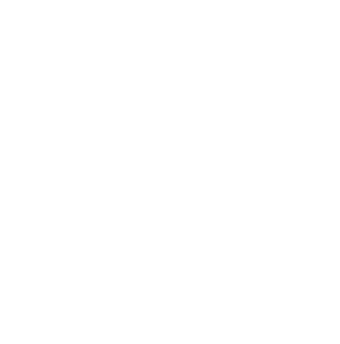
\includegraphics[width=0.3\linewidth,transparent]{parents-boy.png}
  
\includegraphics[width=0.3\linewidth,transparent]{parents-girl.png}
\end{frame}

\begin{frame}
  \frametitle{Sequencing method}

  \vspace{\baselineskip}

  \begin{itemize}
    \item Illumina HiSeq
    \item Full-genome
    \item 500M paired reads of 90bp
    \item 12x average coverage
  \end{itemize}

  \vspace{0.5\baselineskip}

  \begin{center}
    
\includegraphics[width=0.35\linewidth,transparent]{hiseq.png}
  \end{center}
\end{frame}

\section{Sample processing}

\begin{frame}
  Pipeline developed at UMCG based on the BROAD (GATK) pipeline.

  \vspace{\baselineskip}

  120GB per sample.
\end{frame}

\begin{frame}
  Done in about 5 weeks from now.

  \vspace{\baselineskip}

  On UMCG millipede cluster, Sara grid, Rotterdam, Hubrecht, ...
\end{frame}

\section{Quality control}

\begin{frame}
  \frametitle{SNP call concordance}

  Work of Laurent.

  Validate results against our owen pipeline.
\end{frame}

\section{Mitochondrion}

\begin{frame}
  \frametitle{Analysis}
\end{frame}

\section{Y chromosome}

\begin{frame}
  \frametitle{Analysis}
\end{frame}

\section{Questions?}

\lastpagetemplate
\begin{frame}
  \begin{center}
    Acknowledgements:
    \bigskip
    \bigskip

  \end{center}
\end{frame}

\end{document}
